\chapter{Avoiding Burnout: Energy, Sales, and the Word No}

This interview segment is short, but it has a clear internal mechanics. It begins with a direct question about burnout and motivation, then answers by treating energy as a finite operating resource. The speaker's sequence is important: first control energy and emotion, then notice how ordinary communications and decisions drain the day's reserve, then apply the rule commercially. In business, leadership, real estate, and sales, the practical conclusion is that no is not a mood. It is an allocation rule.

\section{The Opening Question}

The question that starts the segment is simple: how do we avoid burnout, and what keeps us motivated? The answer does not begin with inspiration, goals, or discipline. It begins with control. Burnout is described as what happens when a person does not control energy and emotions.

That gives us the structure of the chapter. We are not building a clinical theory of burnout. We are extracting an operator's model: a person begins the day with finite capacity, spends that capacity through contact with the world, and must decide which contacts deserve access to it.

\subsection{Question \& Answer}

\paragraph{Question.}
How do we avoid burnout, and what keeps us motivated?

\paragraph{Answer.}
By controlling energy and emotion before the day spends them for us. In the speaker's account, burnout is not caused by work in the abstract. It is caused by allowing every communication, interaction, and decision to draw from the same limited reserve without a value test.

\section{Burnout As A Control Problem}

The first claim is deliberately narrow. Burnout happens when we fail to control two linked resources:
\begin{itemize}
\item energy, the finite capacity to act, respond, decide, and continue;
\item emotion, the internal state that can make the same interaction either manageable or expensive.
\end{itemize}

We can express the claim with a modest bookkeeping model. Let \(E_0\) denote the usable energy available at the beginning of a day. The lecture does not assign units to \(E_0\), and the notation should not pretend otherwise. It only records the spoken premise that the reserve is finite.

If the day contains demands indexed by \(i\), and if \(c_i\) denotes the energy cost of the \(i\)-th demand, then the remaining energy is reconstructed as
\begin{equation}
E_{\mathrm{remain}}
=
E_0-\sum_i c_i .
\end{equation}

This is not a measured law. It is the mathematical skeleton of the speaker's reasoning: each demand may be small, but the sum is what matters.

\section{The Daily Energy Budget}

The lecture then unfolds the drain in order. We wake up with a certain amount of energy. Then communication begins. Interactions begin. Decisions begin. Each one drains a little bit.

To keep those categories visible, we can separate the total cost into three sums:
\begin{equation}
E_{\mathrm{remain}}
=
E_0
-
\sum_j C_j
-
\sum_k I_k
-
\sum_{\ell} D_{\ell}.
\end{equation}

Here \(C_j\) is the cost of communication \(j\), \(I_k\) is the cost of interaction \(k\), and \(D_{\ell}\) is the cost of decision \(\ell\). The separation is useful because it preserves the rhythm of the interview. The speaker is not saying that one dramatic event creates burnout. He is pointing to repeated small withdrawals.

\begin{figure}
\centering
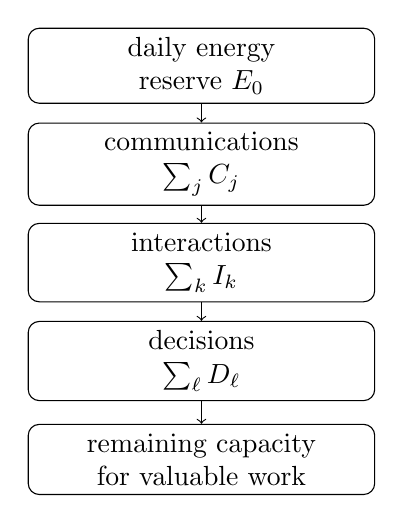
\begin{tikzpicture}[x=1cm,y=1cm]
\node[draw, rounded corners, align=center, minimum width=4.4cm, minimum height=0.75cm] (start) at (0,0) {daily energy\\reserve \(E_0\)};
\node[draw, rounded corners, align=center, minimum width=4.4cm, minimum height=0.75cm] (comm) at (0,-1.25) {communications\\\(\sum_j C_j\)};
\node[draw, rounded corners, align=center, minimum width=4.4cm, minimum height=0.75cm] (inter) at (0,-2.50) {interactions\\\(\sum_k I_k\)};
\node[draw, rounded corners, align=center, minimum width=4.4cm, minimum height=0.75cm] (dec) at (0,-3.75) {decisions\\\(\sum_{\ell}D_{\ell}\)};
\node[draw, rounded corners, align=center, minimum width=4.4cm, minimum height=0.75cm] (remain) at (0,-5.00) {remaining capacity\\for valuable work};

\draw[->] (start) -- (comm);
\draw[->] (comm) -- (inter);
\draw[->] (inter) -- (dec);
\draw[->] (dec) -- (remain);
\end{tikzpicture}
\caption{A transcript-derived reconstruction of the lecture's energy-budget mechanism. The lecture presents the mechanism verbally rather than as a board diagram.}
\end{figure}

\section{The Commercial Pivot: Everyone Is In Sales}

Once the daily reserve is on the table, the speaker pivots to entrepreneurship. If we are business owners, leaders, in real estate, or simply operating commercially, then we are in sales. This is the hinge of the segment.

The point is broader than a job title. Sales means repeated human contact under conditions of attention, persuasion, judgment, and response. Every interaction asks for a piece of the day's reserve. So the sales environment makes the energy budget more urgent: the more people and opportunities enter the system, the more carefully we must decide what deserves a yes.

Let \(r\) denote an incoming request, opportunity, meeting, conversation, or demand on attention. Let \(c(r)\) be the cost of engaging with it, and let \(V(r)\) be the value it adds to the person, the business, or the team. Then the phrase ``worth your time'' can be reconstructed as the decision rule
\begin{equation}
\mathrm{Engage}(r)=1
\quad\Longleftrightarrow\quad
V(r)>c(r).
\end{equation}

The companion rule is
\begin{equation}
\mathrm{Decline}(r)=1
\quad\Longleftrightarrow\quad
V(r)\leq c(r).
\end{equation}

These formulas are deliberately simple. They should be read as a translation of the lecture's operating rule, not as a quantitative sales model.

\section{The Rule Of No}

The conclusion follows naturally: the word no becomes more important. In this model, no is not merely refusal. It is the mechanism that prevents low-value demands from consuming the reserve needed for valuable work.

A short numerical example makes the bookkeeping concrete. Suppose a day begins with
\begin{equation}
E_0=100
\end{equation}
units of usable energy. The units are artificial; only the arithmetic matters. Suppose the known costs are
\begin{equation}
\sum_j C_j=20,
\qquad
\sum_k I_k=35,
\qquad
\sum_{\ell}D_{\ell}=25.
\end{equation}

Then
\begin{align}
E_{\mathrm{remain}}
&=
100-20-35-25 \\
&=
20.
\end{align}

Now suppose one more interaction \(r\) costs \(c(r)=15\), but adds only \(V(r)=5\) units of value to the person, the business, or the team. Then
\begin{equation}
V(r)<c(r),
\end{equation}
so the reconstructed rule says to decline it. The reason is not that interaction is bad. The reason is that this interaction would reduce the remaining reserve from \(20\) to \(5\), leaving little capacity for work that matters more.

Thus the word no protects the day's remaining capacity. It keeps the operator from spending scarce energy on activity that does not add value.

\section{A Cautious Threshold Picture}

The transcript does not give a diagnostic threshold for burnout. Still, its logic points to a qualitative danger condition:
\begin{equation}
\sum_i c_i \gg E_0.
\end{equation}

This should be read only as a warning picture. If accumulated communication, interaction, and decision costs greatly exceed the controlled daily reserve, then the person is no longer allocating energy deliberately. The demands of the day are doing the allocation.

The emotional part of the answer belongs here as well. Two outwardly similar interactions need not have the same cost. A controlled response may keep the cost small; a reactive response may make it larger. As a cautious reconstruction:
\begin{equation}
c_i^{\mathrm{reactive}}
>
c_i^{\mathrm{controlled}}.
\end{equation}

That inequality captures the lecture's opening claim without overstating it. Emotional control does not remove all cost, but it changes how expensive each demand becomes.

\section{Summary}

The segment has a tight progression. It starts with the question of burnout and motivation. It answers by naming control of energy and emotion. It then builds a daily reserve model in which communications, interactions, and decisions drain finite capacity. The business pivot matters because operators live inside repeated sales-like exchanges. The final rule is therefore practical and precise: say no to demands that do not add value to you, your business, or your team, because every unnecessary yes spends energy that cannot be used twice.